\section{Constitutive Laws \label{sect:smm:CL}}\index{Material}
In order to compute an element's response to deformation, one needs to
use an appropriate constitutive relationship. The constitutive law is
used to compute the element's stresses from the element's strains.

In the finite-element discretization, the constitutive formulation is
applied to every quadrature point of each element. When the implicit
formulation is used, the tangent matrix has to be computed.

The chosen materials for the simulation have to be specified in the
mesh file or, as an alternative, they can be assigned using the
\code{element\_material} vector.  For every material assigned to the
problem one has to specify the material characteristics (constitutive
behavior and material properties) in a text file (\eg material.dat) as
follows:
\begin{cpp}
  material %\emph{constitutive\_law}% %\emph{<optional flavor>}% [
     name = $value$
     rho = $value$
     ...
  ]
\end{cpp}
\index{Constitutive\_laws} where \emph{constitutive\_law} is the adopted
constitutive law, followed by the material properties listed one by line in the
bracket (\eg \code{name} and density \code{rho}). Some constitutive laws can
also have an \emph{optional flavor}. For example a non-local constitutive law
can be flavored by a weight function. The file needs to be loaded in \akantu
using the \code{initialize} method of \akantu (as shown in
Section~\ref{sec:writing_main})
\begin{cpp}
  initialize("material.dat", argc, argv);
\end{cpp}
% or, alternatively, the \code{initFull} method.
% \begin{cpp}
%   model.initFull("material.dat");
% \end{cpp}

In order to conveniently store values at each quadrature in a material
point \akantu provides a special data structure, the
\code{InternalField}. The internal fields are inheriting from the
\code{ElementTypeMapArray}.  Furthermore, it provides several functions for
initialization, auto-resizing and auto removal of quadrature points.

Sometimes it is also desired to generate random distributions of
internal parameters. An example might be the critical stress at which the
material fails. To generate such a field, in the material input file,
a random quantity needs be added to the base value:
\begin{cpp}
  sigma_c = $base$
  sigma_c = $base$ uniform [$min$, $max$]
  sigma_c = $base$ weibull [$\lambda$, $m$]
\end{cpp}

All parameters are real numbers. For the uniform distribution, minimum
and maximum values have to be specified.
Random parameters are defined as a $base$ value to which we add a random number
that follows the chosen distribution.

The
\href{http://en.wikipedia.org/wiki/Uniform\_distribution\_(continuous)}{\emph{Uniform}}
distribution is gives a random values between in $[min, max)$. The
\href{http://en.wikipedia.org/wiki/Weibull\_distribution}{\emph{Weibull}}
distribution is characterized by the following cumulative distribution
function:
\begin{equation}
  F(x) = 1- e^{-\left({x/\lambda}\right)^m}
\end{equation}
which depends on  $m$ and $\lambda$, which are the shape parameter and the scale
parameter. These random distributions are different each time the code
is executed. In order to obtain always the same one, it possible to
manually set the \emph{seed} that is the number from which these
pseudo-random distributions are created. This can be done by adding
the following line to the input file \emph{outside} the material
parameters environments:
\begin{cpp}
  seed = 1.0
\end{cpp}
where the value 1 can be substituted with any number. Currently
\akantu is can reproduce always the same distribution when the seed is
specified \emph{only} in serial.

The following sections describe the constitutive models implemented in
\akantu. In Appendix~\ref{app:material-parameters} a summary of the
parameters for all materials of \akantu is provided.


\subsection{Elasticity}\index{Material!Elastic}

The elastic law is a commonly used constitutive relationship that can be used
for a wide range of engineering materials (\eg metals, concrete, rock, wood,
glass, rubber, etc.) provided that the strains remain small (\ie small
deformation and stress lower than yield strength).

The elastic laws are often expressed as $\mat{\sigma} =
\mat{C}:\mat{\varepsilon}$ with where $\mat{\sigma}$ is the Cauchy stress tensor,
$\mat{\varepsilon}$ represents the infinitesimal strain tensor and $\mat{C}$ is the
elastic modulus tensor.

\subsubsection{Linear isotropic\matlabel{ssect:smm:linear-elastic-isotropic}}

The linear isotropic elastic behavior is described by Hooke's law, which states
that the stress is linearly proportional to the applied strain (material behaves
like an ideal spring), as illustrated in Figure~\ref{fig:smm:cl:elastic}.
\begin{figure}[!htb]
  \begin{center}

    \subfloat[]{
      \begin{tikzpicture}
	\draw[thick,latex-latex] (0,5) node[left] {$\sigma$} |- (5,0) node (x) [right, below] {$\varepsilon$};
	\draw[thin] (1.5,1.5) -- (2.5,1.5) -- (2.5,2.5) node [midway, right] {E};
	\draw[very thick,color=red] (0,0) -- (4,4);
	\draw[very thick,latex-latex,color=red] (1,1) -- (3,3);
      \end{tikzpicture}
      \label{fig:smm:cl:elastic:stress_strain} }
    \hspace{0.05\textwidth} \subfloat[]{
      \raisebox{0.125\textwidth}{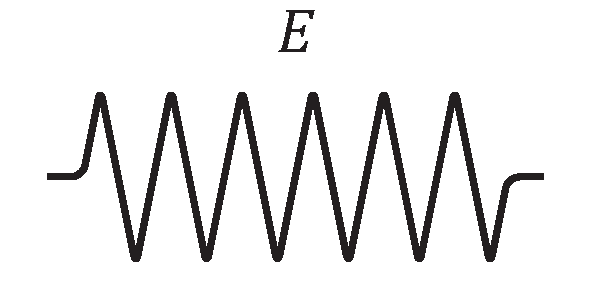
\includegraphics[width=0.25\textwidth,keepaspectratio=true]{figures/hooke_law.pdf}}
      \label{fig:smm:cl:elastic:hooke} }
    \caption{(a) Stress-strain curve for elastic material and (b)
      schematic representation of Hooke's law, denoted as a spring.}
    \label{fig:smm:cl:elastic}
  \end{center}
\end{figure}
The equation that relates the strains to the
displacements is: % First the strain is computed (at every gauss
point) from the displacements as follows:
\begin{equation}
  \label{eqn:smm:strain_inf}
  \mat{\varepsilon} =
  \frac{1}{2} \left[ \nabla_0 \vec{u}+\nabla_0 \vec{u}^T \right]
\end{equation}
where $\mat{\varepsilon}$ represents the infinitesimal strain tensor,
$\nabla_{0}\vec{u}$ the displacement gradient
tensor according to the initial configuration. The constitutive equation
for isotropic homogeneous media can be expressed as:
\begin{equation}
  \label{eqn:smm:material:constitutive_elastic}
  \mat{\sigma } =\lambda\mathrm{tr}(\mat{\varepsilon})\mat{I}+2 \mu\mat{\varepsilon}
\end{equation}
where $\mat{\sigma}$ is the Cauchy stress tensor
($\lambda$ and $\mu$ are the the first and second Lame's
coefficients).

In Voigt notation this correspond to
\begin{align}
  \left[\begin{array}{c}
      \sigma_{11}\\
      \sigma_{22}\\
      \sigma_{33}\\
      \sigma_{23}\\
      \sigma_{13}\\
      \sigma_{12}\\
    \end{array}\right]
  &= \frac{E}{(1+\nu)(1-2\nu)}\left[
    \begin{array}{cccccc}
      1-\nu & \nu   & \nu   & 0 & 0 & 0\\
      \nu   & 1-\nu & \nu   & 0 & 0 & 0\\
      \nu   & \nu   & 1-\nu & 0 & 0 & 0\\
      0     &  0    &  0    & \frac{1-2\nu}{2} & 0 & 0 \\
      0     &  0    &  0    & 0 & \frac{1-2\nu}{2} & 0 \\
      0     &  0    &  0    & 0 & 0 & \frac{1-2\nu}{2} \\
    \end{array}\right]
  \left[\begin{array}{c}
      \varepsilon_{11}\\
      \varepsilon_{22}\\
      \varepsilon_{33}\\
      2\varepsilon_{23}\\
      2\varepsilon_{13}\\
      2\varepsilon_{12}\\
    \end{array}\right]
\end{align}

\subsubsection{Linear anisotropic\matlabel{ssect:smm:linear-elastic-anisotropic}}
This formulation is not sufficient to represent all elastic material
behavior. Some materials have characteristic orientation that have to be taken
into account. To represent this anisotropy a more general stress-strain law has
to be used. For this we define the elastic modulus tensor as follow:

\begin{align}
  \left[\begin{array}{c}
      \sigma_{11}\\
      \sigma_{22}\\
      \sigma_{33}\\
      \sigma_{23}\\
      \sigma_{13}\\
      \sigma_{12}\\
    \end{array}\right]
  &= \left[
    \begin{array}{cccccc}
      c_{11} & c_{12} & c_{13} & c_{14} & c_{15} & c_{16}\\
      c_{21} & c_{22} & c_{23} & c_{24} & c_{25} & c_{26}\\
      c_{31} & c_{32} & c_{33} & c_{34} & c_{35} & c_{36}\\
      c_{41} & c_{42} & c_{43} & c_{44} & c_{45} & c_{46}\\
      c_{51} & c_{52} & c_{53} & c_{54} & c_{55} & c_{56}\\
      c_{61} & c_{62} & c_{63} & c_{64} & c_{65} & c_{66}\\
    \end{array}\right]
  \left[\begin{array}{c}
      \varepsilon_{11}\\
      \varepsilon_{22}\\
      \varepsilon_{33}\\
      2\varepsilon_{23}\\
      2\varepsilon_{13}\\
      2\varepsilon_{12}\\
    \end{array}\right]
\end{align}

\begin{figure}[h]
  \centering
  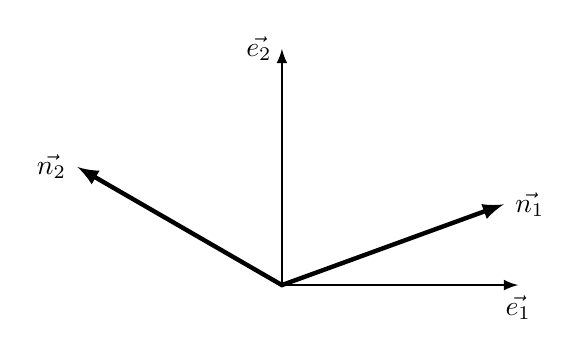
\begin{tikzpicture}
    \draw[thick,latex-latex] (90:3) node[left] {$\vec{e_2}$} |- (0:3) node [right, below] {$\vec{e_1}$};
    \draw[ultra thick,latex-latex] (150:3) node[left] {$\vec{n_2}$} -- (0,0) -- (20:3) node [right] {$\vec{n_1}$};
  \end{tikzpicture}
  \caption{Material basis}
\end{figure}

To simplify the writing of input files the \mat{C} tensor is expressed in the
material basis. And this basis as to be given too. This basis $\Omega_{\st{mat}}
= \{\vec{n_1}, \vec{n_2}, \vec{n_3}\}$ is used to define the rotation $R_{ij} =
\vec{n_j} . \vec{e_i}$. And $\mat{C}$ can be rotated in the global basis $\Omega
= \{\vec{e_1}, \vec{e_2}, \vec{e_3}\}$ as follow:


\begin{align}
\mat{C}_{\Omega} &= \mat{R}_1 \mat{C}_{\Omega_{\st{mat}}} \mat{R}_2\\
\mat{R}_1  &= \left[
  \begin{array}{cccccc}
    R_{11} R_{11} & R_{12} R_{12} & R_{13} R_{13} & R_{12} R_{13} & R_{11} R_{13} & R_{11} R_{12}\\
    R_{21} R_{21} & R_{22} R_{22} & R_{23} R_{23} & R_{22} R_{23} & R_{21} R_{23} & R_{21} R_{22}\\
    R_{31} R_{31} & R_{32} R_{32} & R_{33} R_{33} & R_{32} R_{33} & R_{31} R_{33} & R_{31} R_{32}\\
    R_{21} R_{31} & R_{22} R_{32} & R_{23} R_{33} & R_{22} R_{33} & R_{21} R_{33} & R_{21} R_{32}\\
    R_{11} R_{31} & R_{12} R_{32} & R_{13} R_{33} & R_{12} R_{33} & R_{11} R_{33} & R_{11} R_{32}\\
    R_{11} R_{21} & R_{12} R_{22} & R_{13} R_{23} & R_{12} R_{23} & R_{11} R_{23} & R_{11} R_{22}\\
  \end{array}\right]\\
\mat{R}_2  &= \left[
  \begin{array}{cccccc}
    R_{11} R_{11} & R_{21} R_{21} & R_{31} R_{31} & R_{21} R_{31} & R_{11} R_{31} & R_{11} R_{21}\\
    R_{12} R_{12} & R_{22} R_{22} & R_{32} R_{32} & R_{22} R_{32} & R_{12} R_{32} & R_{12} R_{22}\\
    R_{13} R_{13} & R_{23} R_{23} & R_{33} R_{33} & R_{23} R_{33} & R_{13} R_{33} & R_{13} R_{23}\\
    R_{12} R_{13} & R_{22} R_{23} & R_{32} R_{33} & R_{22} R_{33} & R_{12} R_{33} & R_{12} R_{23}\\
    R_{11} R_{13} & R_{21} R_{23} & R_{31} R_{33} & R_{21} R_{33} & R_{11} R_{33} & R_{11} R_{23}\\
    R_{11} R_{12} & R_{21} R_{22} & R_{31} R_{32} & R_{21} R_{32} & R_{11} R_{32} & R_{11} R_{22}\\
  \end{array}\right]\\
\end{align}

\subsubsection{Linear orthotropic\matlabel{ssect:smm:linear-elastic-orthotropic}}

A particular case of anisotropy is when the material basis is orthogonal in which case the elastic modulus tensor can be simplified and rewritten in terms of 9 independents material parameters.

\begin{align}
  \left[\begin{array}{c}
      \sigma_{11}\\
      \sigma_{22}\\
      \sigma_{33}\\
      \sigma_{23}\\
      \sigma_{13}\\
      \sigma_{12}\\
    \end{array}\right]
  &= \left[
    \begin{array}{cccccc}
      c_{11} & c_{12} & c_{13} &   0   &   0   &   0  \\
            & c_{22} & c_{23} &   0   &   0   &   0  \\
            &       & c_{33} &   0   &   0   &   0  \\
            &       &       & c_{44} &   0   &   0  \\
            &  \multicolumn{2}{l}{\text{sym.}}       &       & c_{55} &   0  \\
            &       &       &       &       & c_{66}\\
    \end{array}\right]
  \left[\begin{array}{c}
      \varepsilon_{11}\\
      \varepsilon_{22}\\
      \varepsilon_{33}\\
      2\varepsilon_{23}\\
      2\varepsilon_{13}\\
      2\varepsilon_{12}\\
    \end{array}\right]
\end{align}

\begin{align}
  c_{11} &= E_1 (1 - \nu_{23}\nu_{32})\Gamma \qquad c_{22} = E_2 (1 - \nu_{13}\nu_{31})\Gamma \qquad c_{33} = E_3 (1 - \nu_{12}\nu_{21})\Gamma\\
  c_{12} &= E_1 (\nu_{21} - \nu_{31}\nu_{23})\Gamma = E_2 (\nu_{12} - \nu_{32}\nu_{13})\Gamma\\
  c_{13} &= E_1 (\nu_{31} - \nu_{21}\nu_{32})\Gamma = E_2 (\nu_{13} - \nu_{21}\nu_{23})\Gamma\\
  c_{23} &= E_2 (\nu_{32} - \nu_{12}\nu_{31})\Gamma = E_3 (\nu_{23} - \nu_{21}\nu_{13})\Gamma\\
  c_{44} &= \mu_{23} \qquad  c_{55} = \mu_{13} \qquad  c_{66} = \mu_{12} \\
  \Gamma &= \frac{1}{1 - \nu_{12} \nu_{21} - \nu_{13} \nu_{31} - \nu_{32} \nu_{23} - 2 \nu_{21} \nu_{32} \nu_{13}}
\end{align}

The Poisson ratios follow the rule $\nu_{ij} = \nu_{ji} E_i / E_j$.

\subsection{Neo-Hookean\matlabel{ssect:smm:cl:neohookean}}\index{Material!Neohookean}
The hyperelastic Neo-Hookean constitutive law results from an
extension of the linear elastic relationship (Hooke's Law) for large
deformation. Thus, the model predicts nonlinear stress-strain behavior
for bodies undergoing large deformations.

\begin{figure}[!htb]
  \begin{center}
    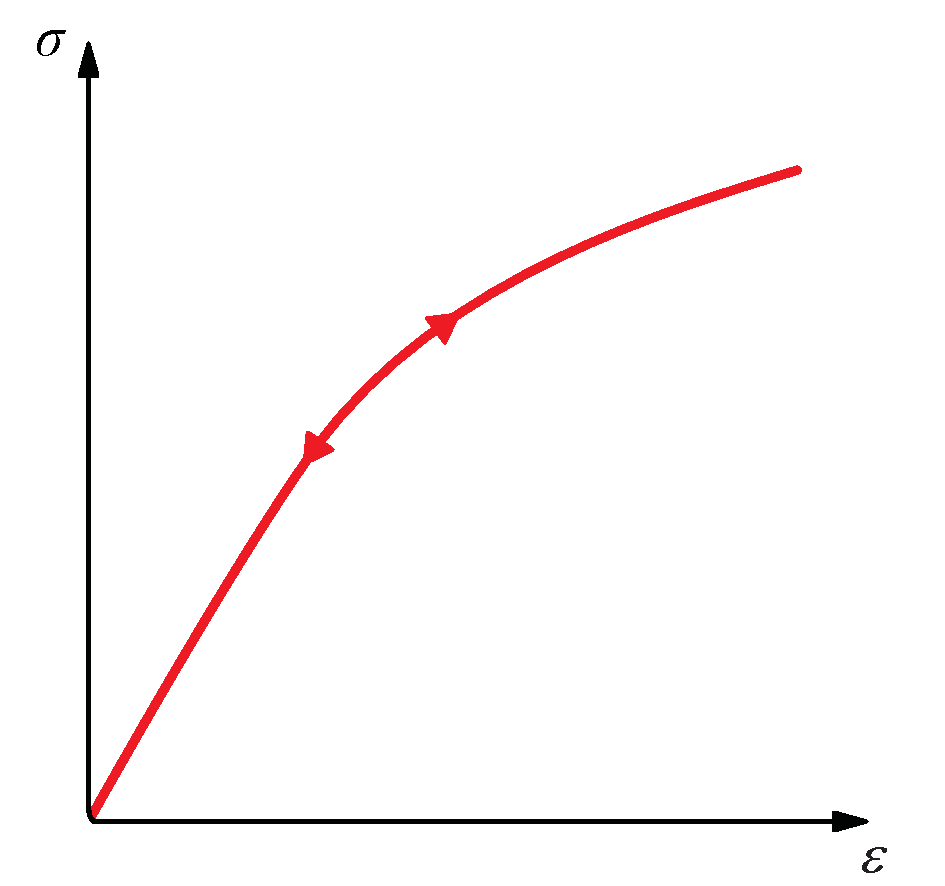
\includegraphics[width=0.4\textwidth,keepaspectratio=true]{figures/stress_strain_neo.pdf}
    \caption{Neo-hookean Stress-strain curve.}
    \label{fig:smm:cl:neo_hookean}
  \end{center}
\end{figure}

As illustrated in Figure~\ref{fig:smm:cl:neo_hookean}, the behavior is initially
linear and the mechanical behavior is very close to the corresponding linear
elastic material. This constitutive relationship, which accounts for compressibility,
is a modified version of the one proposed by Ronald Rivlin \cite{Belytschko:2000}.

The strain energy stored in the material is given by:
\begin{equation}\label{eqn:smm:constitutive:neohookean_potential}
  \Psi(\mat{C}) = \frac{1}{2}\lambda_0\left(\ln J\right)^2-\mu_0\ln J+\frac{1}{2}
  \mu_0\left(\mathrm{tr}(\mat{C})-3\right)
\end{equation}
\noindent where $\lambda_0$ and $\mu_0$ are, respectively, Lam\'e's first parameter
and the shear modulus at the initial configuration. $J$ is the jacobian of the deformation
gradient ($\mat{F}=\nabla_{\!\!\vec{X}}\vec{x}$): $J=\text{det}(\mat{F})$. Finally $\mat{C}$ is the right Cauchy-Green
deformation tensor.

Since this kind of material is used for large deformation problems, a
finite deformation framework should be used. Therefore, the Cauchy
stress ($\mat{\sigma}$) should be computed through the second
Piola-Kirchhoff stress tensor $\mat{S}$:

\begin{equation}
  \mat{\sigma } = \frac{1}{J}\mat{F}\mat{S}\mat{F}^T
\end{equation}

Finally the second Piola-Kirchhoff stress tensor is given by:

\begin{equation}
  \mat{S}  = 2\frac{\partial\Psi}{\partial\mat{C}} = \lambda_0\ln J
  \mat{C}^{-1}+\mu_0\left(\mat{I}-\mat{C}^{-1}\right)
\end{equation}

The parameters to indicate in the material file are the same
as those for the elastic case: \code{E} (Young's modulus), \code{nu} (Poisson's
ratio).


\subsection{Visco-Elasticity\matlabel{ssect:smm:cl:sls}}
% Standard Solid rheological model, see [] J.C. Simo, T.J.R. Hughes,
% "Computational Inelasticity", Springer (1998), see Sections 10.2 and 10.3
Visco-elasticity is characterized by strain rate dependent
behavior. Moreover, when such a material undergoes a deformation it
dissipates energy. This dissipation results in a hysteresis loop in
the stress-strain curve at every loading cycle (see
Figure~\ref{fig:smm:cl:visco-elastic:hyst}). In principle, it can be
applied to many materials, since all materials exhibit a visco-elastic
behavior if subjected to particular conditions (such as high
temperatures).
\begin{figure}[!htb]
  \begin{center}

    \subfloat[]{
      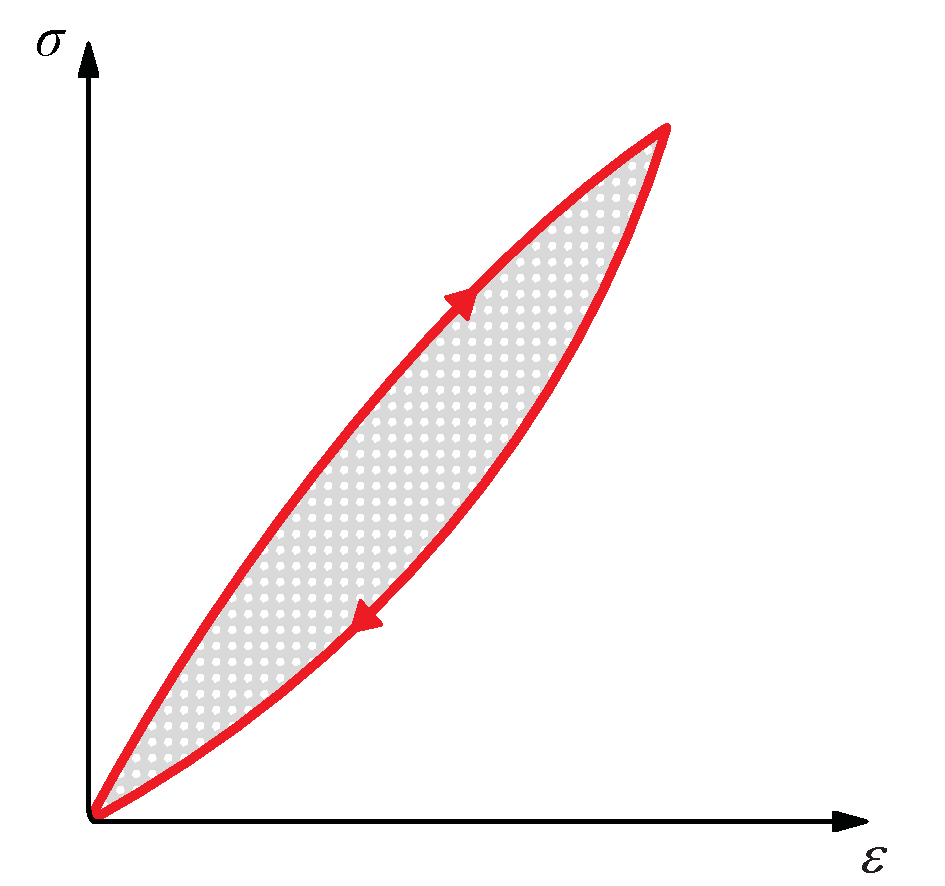
\includegraphics[width=0.4\textwidth,keepaspectratio=true]{figures/stress_strain_visco.pdf}
      \label{fig:smm:cl:visco-elastic:hyst}
    }
    \hspace{0.05\textwidth}
    \subfloat[]{
      \raisebox{0.025\textwidth}{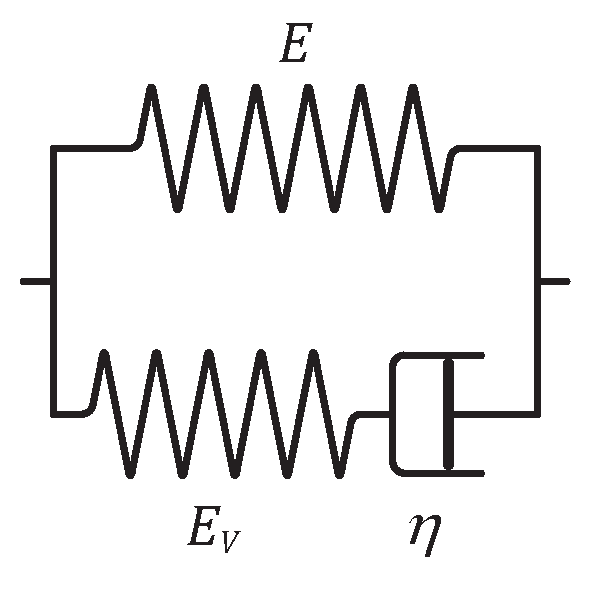
\includegraphics[width=0.3\textwidth,keepaspectratio=true]{figures/visco_elastic_law.pdf}}
      \label{fig:smm:cl:visco-elastic:model}
    }
    \caption{(a) Characteristic stress-strain behavior of a visco-elastic material with hysteresis loop and (b) schematic representation of the standard rheological linear solid visco-elastic model.}
    \label{fig:smm:cl:visco-elastic}
  \end{center}
\end{figure}
The standard rheological linear solid model (see Sections 10.2 and 10.3
of~\cite{simo92}) has been implemented in \akantu. This model results from the
combination of a spring mounted in parallel with a spring and a dashpot
connected in series, as illustrated in
Figure~\ref{fig:smm:cl:visco-elastic:model}. The advantage of this model is that
it allows to account for creep or stress relaxation. The equation that relates
the stress to the strain is (in 1D):
\begin{equation}
  \frac{d\varepsilon(t)}{dt} = \left ( E + E_V \right ) ^ {-1} \cdot \left [ \frac{d\sigma(t)}{dt} + \frac{E_V}{\eta}\sigma(t) - \frac{EE_V}{\eta}\varepsilon(t) \right ]
\end{equation}
where $\eta$ is the viscosity. The equilibrium condition is unique and
is attained in the limit, as $t \to \infty $. At this stage, the
response is elastic and depends on the Young's modulus $E$.  The
mandatory parameters for the material file are the following:
\code{rho} (density), \code{E} (Young's modulus), \code{nu} (Poisson's
ratio), \code{Plane\_Stress} (if set to zero plane strain, otherwise
plane stress), \code{eta} (dashpot viscosity) and \code{Ev} (stiffness
of the viscous element).

Note that the current standard linear solid model is applied only on the deviatoric part of the strain tensor. The spheric part of the strain tensor affects the stress tensor like an linear elastic material.

\subsection{Small-Deformation Plasticity\matlabel{ssect:smm:cl:plastic}}\index{Material!Small-deformation Plasticity}
The small-deformation plasticity is a simple plasticity material
formulation which accounts for the additive decomposition of strain
into elastic and plastic strain components. This formulation is
applicable to infinitesimal deformation where the additive
decomposition of the strain is a valid approximation. In this
formulation, plastic strain is a shearing process where hydrostatic
stress has no contribution to plasticity and consequently plasticity
does not lead to volume change. Figure~\ref{fig:smm:cl:Lin-strain-hard}
shows the linear strain hardening elasto-plastic behavior according to
the additive decomposition of strain into the elastic and plastic
parts in infinitesimal deformation as
\begin{align}
  \mat{\varepsilon} &= \mat{\varepsilon}^e +\mat{\varepsilon}^p\\
  {\mat{\sigma}} &= 2G(\mat{\varepsilon}^e) + \lambda  \mathrm{tr}(\mat{\varepsilon}^e)\mat{I}
\end{align}

\begin{figure}[htp]
  \centering
  {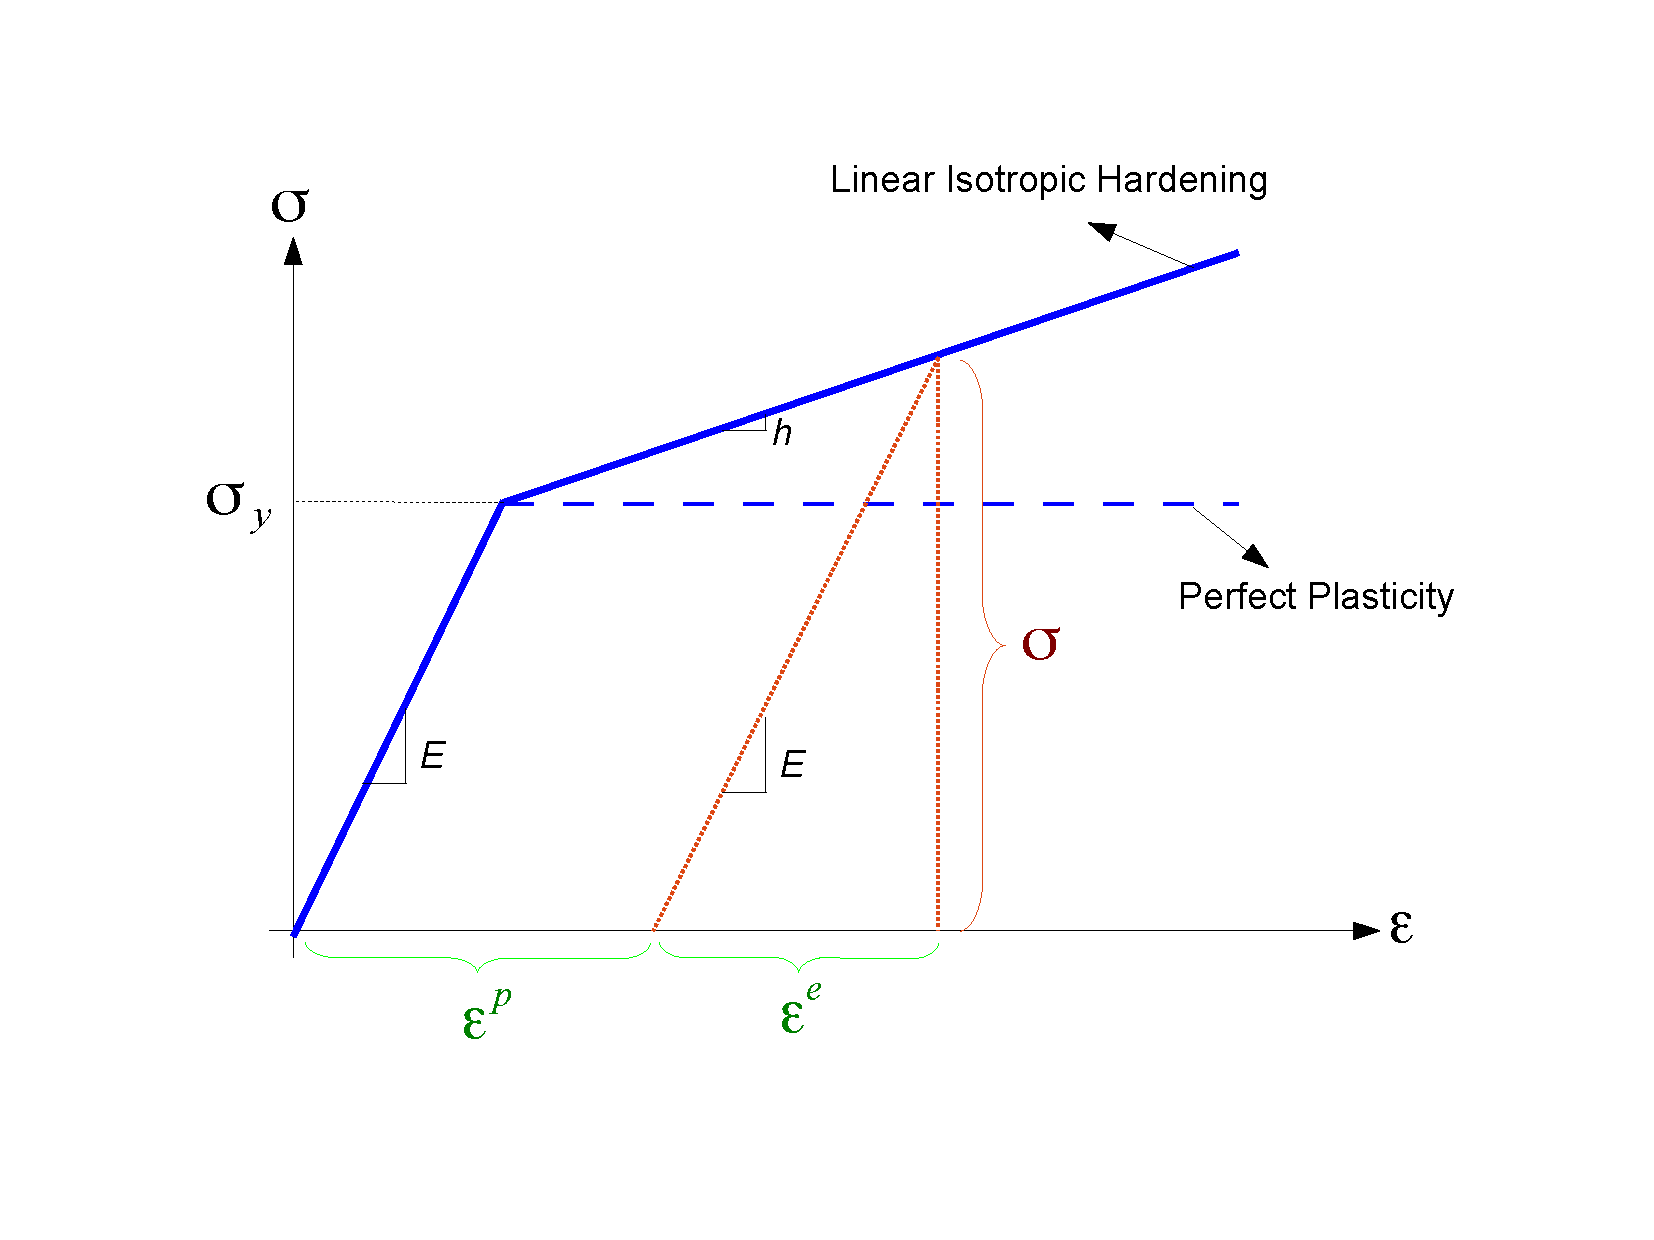
\includegraphics[scale=0.4, clip]{figures/isotropic_hardening_plasticity.pdf}}
  \caption{
    Stress-strain curve for the small-deformation plasticity with linear isotropic hardening.
  }
  \label{fig:smm:cl:Lin-strain-hard}
\end{figure}

\noindent In this class, the von Mises yield criterion is used. In the von Mises yield criterion, the yield is independent of the hydrostatic stress. Other yielding criteria such as Tresca and Gurson can be easily implemented in this class as well.

In the von Mises yield criterion, the hydrostatic stresses have no effect on the plasticity and consequently the yielding occurs when a critical elastic shear energy is achieved.
\begin{equation} \label{eqn:smm:constitutive:von Mises}
  f = \sigma_{\st{eff}} - \sigma_y = \left(\frac{3}{2} {\mat{\sigma}}^{\st{tr}} : {\mat{\sigma}}^{\st{tr}}\right)^\frac{1}{2}-\sigma_y (\mat{\varepsilon}^p)
\end{equation}
\begin{equation} \label{eqn:smm:constitutive:yielding}
  f < 0 \quad \textrm{Elastic deformation,} \qquad f = 0 \quad  \textrm{Plastic deformation}
\end{equation}
where $\sigma_y$ is the yield strength of the material which can be function of plastic strain in case of hardening type of materials and ${\mat{\sigma}}^{\st{tr}}$ is the deviatoric part of stress given by
\begin{equation} \label{eqn:smm:constitutive:deviatoric stress}
  {\mat{\sigma}}^{\st{tr}}=\mat{\sigma} - \frac{1}{3} \mathrm{tr}(\mat{\sigma}) \mat {I}
\end{equation}

After yielding $(f = 0)$, the normality hypothesis of plasticity determines the direction of plastic flow which is normal to the tangent to the yielding surface at the load point. Then, the tensorial form of the plastic constitutive equation using the von Mises yielding criterion (see equation 4.34) may be written as
\begin{equation} \label{eqn:smm:constitutive:plastic contitutive equation}
  \Delta {\mat{\varepsilon}}^p = \Delta p \frac {\partial{f}}{\partial{\mat \sigma}}=\frac{3}{2} \Delta p \frac{{\mat{\sigma}}^{\st{tr}}}{\sigma_{\st{eff}}}
\end{equation}

In these expressions, the direction of the plastic strain increment (or equivalently, plastic strain rate) is given by $\frac{{\mat{\sigma}}^{\st{tr}}}{\sigma_{\st{eff}}}$ while the magnitude is defined by the plastic multiplier $\Delta p$. This can be obtained using the \emph{consistency condition} which impose the requirement for the load point to remain on the yielding surface in the plastic regime.

Here, we summarize the implementation procedures for the
small-deformation plasticity with linear isotropic hardening:
\begin{enumerate}
\item Compute the trial stress:
  \begin{equation}
    {\mat{\sigma}}^{\st{tr}} = {\mat{\sigma}}_t + 2G\Delta \mat{\varepsilon} + \lambda \mathrm{tr}(\Delta \mat{\varepsilon})\mat{I}
  \end{equation}
\item Check the Yielding criteria:
  \begin{equation}
    f = (\frac{3}{2} {\mat{\sigma}}^{\st{tr}} : {\mat{\sigma}}^{\st{tr}})^{1/2}-\sigma_y (\mat{\varepsilon}^p)
  \end{equation}
\item Compute the Plastic multiplier:
  \begin{align}
    d \Delta p &= \frac{\sigma^{tr}_{eff} - 3G \Delta P^{(k)}- \sigma_y^{(k)}}{3G + h}\\
    \Delta p^{(k+1)} &= \Delta p^{(k)}+ d\Delta p\\
    \sigma_y^{(k+1)} &= (\sigma_y)_t+ h\Delta p
  \end{align}
\item Compute the plastic strain increment:
  \begin{equation}
    \Delta {\mat{\varepsilon}}^p = \frac{3}{2} \Delta p \frac{{\mat{\sigma}}^{\st{tr}}}{\sigma_{\st{eff}}}
  \end{equation}
\item Compute the stress increment:
  \begin{equation}
    {\Delta \mat{\sigma}} = 2G(\Delta \mat{\varepsilon}-\Delta \mat{\varepsilon}^p) + \lambda  \mathrm{tr}(\Delta \mat{\varepsilon}-\Delta \mat{\varepsilon}^p)\mat{I}
  \end{equation}
\item Update the variables:
  \begin{align}
    {\mat{\varepsilon^p}} &= {\mat{\varepsilon}}^p_t+{\Delta {\mat{\varepsilon}}^p}\\
    {\mat{\sigma}} &= {\mat{\sigma}}_t+{\Delta \mat{\sigma}}
  \end{align}
\end{enumerate}

We use an implicit integration technique called \emph{the radial
  return method} to obtain the plastic multiplier. This method has the
advantage of being unconditionally stable, however, the accuracy
remains dependent on the step size. The plastic parameters to indicate
in the material file are: \code{$\sigma_y$} (Yield stress) and
\code{h} (Hardening modulus). In addition, the elastic parameters need
to be defined as previously mentioned: \code{E} (Young's modulus),
\code{nu} (Poisson's ratio).

\subsection{Damage}

In the  simplified case of a  linear elastic and brittle  material, isotropic
damage can be represented by a scalar variable $d$, which varies from $0$ to $1$
for  no  damage  to  fully  broken  material  respectively.  The  stress-strain
relationship then becomes:
\begin{equation*}
  \mat{\sigma} = (1-d)\, \mat{C}:\mat{\varepsilon}
\end{equation*}

where  $\mat{\sigma}$,  $\mat{\varepsilon}$ are  the  Cauchy  stress and  strain
tensors, and $\mat{C}$ is the elastic stiffness tensor. This formulation relies
on the definition of an evolution law for the damage variable. In \akantu, many
possibilities exist and they are listed below.

\subsubsection{Marigo\matlabel{ssect:smm:cl:damage-marigo}}

This damage evolution law is energy based as defined by Marigo \cite{marigo81a,
  lemaitre96a}. It is an isotropic damage law.
\begin{align}
  Y &= \frac{1}{2}\mat{\varepsilon}:\mat{C}:\mat{\varepsilon}\\
  F &= Y - Y_d - S d\\
  d &= \left\{
    \begin{array}{l l}
      \mathrm{min}\left(\frac{Y-Y_d}{S},\;1\right) & \mathrm{if}\; F > 0\\
      \mathrm{unchanged} & \mathrm{otherwise}
    \end{array}
  \right.
\end{align}
In this formulation, $Y$ is the strain energy release rate, $Y_d$ the
rupture criterion and $S$ the damage energy.  The non-local version of
this damage evolution law is constructed by averaging the energy $Y$.

\subsubsection{Mazars\matlabel{ssect:smm:cl:damage-mazars}}

This law introduced by Mazars \cite{mazars84a} is a behavioral model to
represent damage evolution in concrete. This model does not rely on the computation of the tangent stiffness, the damage is directly evaluated from the strain.

The governing variable in this damage
law is the equivalent strain $\varepsilon_{\st{eq}} =
\sqrt{<\mat{\varepsilon}>_+:<\mat{\varepsilon}>_+}$, with $<.>_+$ the positive
part of the tensor. This part is defined in the principal coordinates (I, II, III) as $\varepsilon_{\st{eq}} =
\sqrt{<\mat{\varepsilon_I}>_+^2 + <\mat{\varepsilon_{II}}>_+^2 + <\mat{\varepsilon_{III}}>_+^2}$.
The damage is defined as:
\begin{align}
  D &= \alpha_t^\beta D_t + (1-\alpha_t)^\beta D_c\\
  D_t &= 1 - \frac{\kappa_0 (1- A_t)}{\varepsilon_{\st{eq}}} - A_t \exp^{-B_t(\varepsilon_{\st{eq}}-\kappa_0)}\\
  D_c &= 1 - \frac{\kappa_0 (1- A_c)}{\varepsilon_{\st{eq}}} - A_c
  \exp^{-B_c(\varepsilon_{\st{eq}}-\kappa_0)}\\
  \alpha_t &= \frac{\sum_{i=1}^3<\varepsilon_i>_+\varepsilon_{\st{nd}\;i}}{\varepsilon_{\st{eq}}^2}
\end{align}
With $\kappa_0$ the damage threshold, $A_t$ and $B_t$ the damage parameter in
traction, $A_c$ and $B_c$ the damage parameter in compression, $\beta$ is the
shear parameter. $\alpha_t$ is the coupling parameter between traction and
compression, the $\varepsilon_i$ are the eigenstrain and the
$\varepsilon_{\st{nd}\;i}$ are the eigenvalues of the strain if the material
were undamaged.

The coefficients $A$ and $B$ are the post-peak asymptotic
value and the decay shape parameters.

\IfFileExists{manual-constitutive-laws-non_local.tex}{\section{Non-Local Constitutive Laws \label{sect:smm:CLNL}}\index{Material}

Continuum damage modeling of quasi-brittle materials undergo significant softening after the onset of damage. This fast growth of damage causes a loss of ellipticity of partial differential equations of equilibrium. Therefore, the numerical simulation results won't be objective anymore, because the dissipated energy will depend on mesh size used in the simulation. One way to avoid this effect is the use of non-local damage formulations. In this approach a local quantity such as the strain is replaced by its non-local average, where the size of the domain, over which the quantitiy is averaged, depends on the underlying material microstructure. 
\akantu provides non-local versions of many constitutive laws for damage. Examples are for instance the material Mazar and the material Marigo, that can be used in a non-local context. In order to use the corresponding non-local formulation the user has to define the non-local material he wishes to use in the text input file:
\begin{cpp}
  material %\emph{constitutive\_law\_non\_local}% [
     name = %\emph{material\_name}
     rho = $value$
     ...
  ]
\end{cpp}
where \emph{constitutive\_law\_non\_local} is the name of the non-local consitutive law, \textit{e.g.} \emph{marigo\_non\_local}.
In addition to the material the non-local neighborhood, that should be used for the averaging process needs to be defined in the material file as well: 
\begin{cpp}
  non_local %\emph{neighborhood\_name}%  %\emph{weight\_function\_type}% [
     radius = $value$
     ...
      weight_function weight_parameter [
        damage_limit = $value$
        ...
     ]
  ]
\end{cpp}
for the non-local averaging, \textit{e.g.} \emph{base\_wf}, followed by the properties of the non-local neighborhood, such as the radius, and the weight function parameters. It is important to notice that the non-local neighborhood must have the same name as the material to which the neighborhood belongs!
The following two sections list the non-local constitutive laws and different type of weight functions available in \akantu.
\subsection{Non-local constitutive laws}
\textbf{Description to be added!!!}
\subsection{Non-local weight functions}
 \textbf{Description to be added!!!}}{}

\IfFileExists{manual-extra_materials.tex}{% \subsubsection{Caughey}
% ** Not in  release ** The model  is a particular case of  the Rayleigh damping
% model,   with    damping   being   proportional   only    to   the   stiffness
% matrix. Substitute with complete Rayleigh damping model for release?

\subsection{Neo-Hookean}\index{Material!Neohookean}

The hyperelastic Neo-Hookean constitutive law results from an
extension of the linear elastic relationship (Hooke's Law) for large
deformation. Thus, the model predicts nonlinear stress-strain behavior
for bodies undergoing large deformations.

\begin{figure}[!htb]
  \begin{center}
    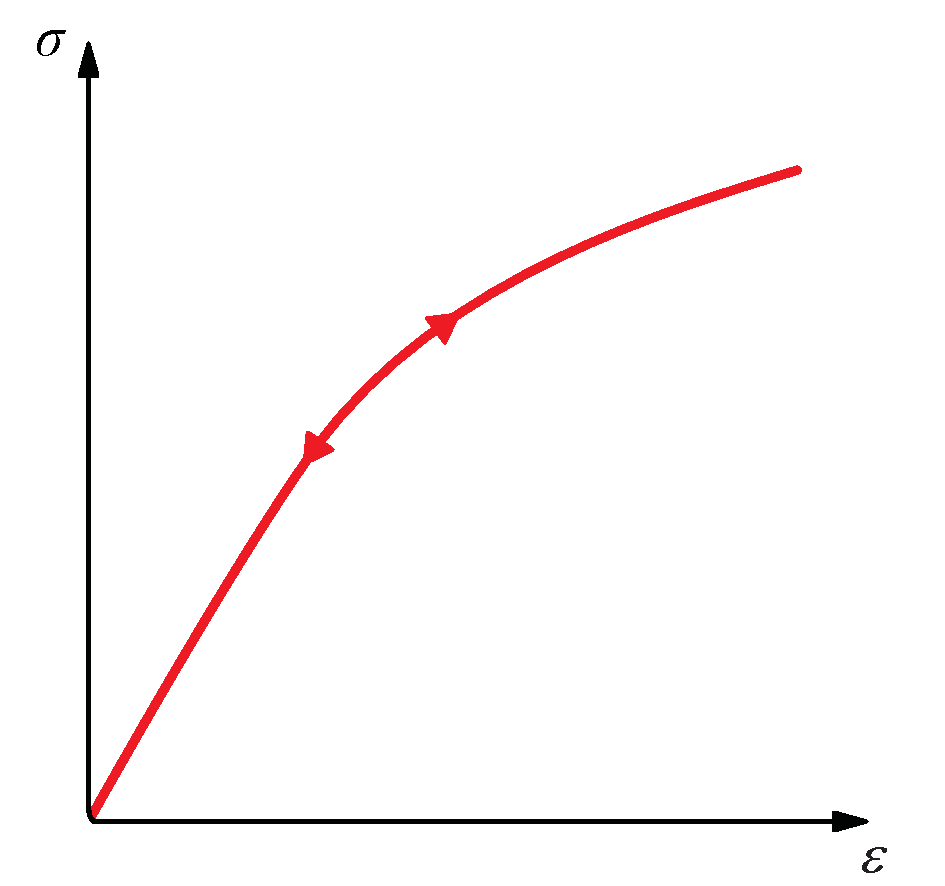
\includegraphics[width=0.4\textwidth,keepaspectratio=true]{figures/stress_strain_neo.pdf}
    \caption{Neo-hookean Stress-strain curve.}
    \label{fig:smm:cl:neo_hookean}
  \end{center}
\end{figure}

As illustrated in Figure~\ref{fig:smm:cl:neo_hookean}, the behavior is initially
linear and the mechanical behavior is very close to the corresponding linear
elastic material. This constitutive relationship, which accounts for compressibility,
 is a modified version of the one proposed by Ronald Rivlin \cite{Belytschko:2000}.

The strain energy stored in the material is given by:
\begin{equation}\label{eqn:smm:constitutive:neohookean_potential}
  \Psi(\mat{C}) = \frac{1}{2}\lambda_0\left(\ln J\right)^2-\mu_0\ln J+\frac{1}{2}
\mu_0\left(\text{trace}(\mat{C})-3\right)
\end{equation}
\noindent where $\lambda_0$ and $\mu_0$ are, respectively, Lamé's first parameter
and the shear modulus at the initial configuration. $J$ is the jacobian of the deformation
gradient ($\mat{F}=\nabla_{\!\!\vec{X}}\vec{x}$): $J=\text{det}(\mat{F})$. Finally $\mat{C}$ is the right Cauchy-Green
deformation tensor.

Since this kind of material is used for large deformation problems, a
finite deformation framework should be used. Therefore, the Cauchy
stress ($\mat{\sigma}$) should be computed through the second
Piola-Kirchhoff stress tensor $\mat{S}$:

\begin{equation}
  \mat{\sigma } = \frac{1}{J}\mat{F}\mat{S}\mat{F}^T
\end{equation}

Finally the second Piola-Kirchhoff stress tensor is given by:

\begin{equation}
  \mat{S}  = 2\frac{\partial\Psi}{\partial\mat{C}} = \lambda_0\ln J
\mat{C}^{-1}+\mu_0\left(\mat{I}-\mat{C}^{-1}\right)
\end{equation}

The parameters to indicate in the material file are the same
as those for the elastic case: \code{E} (Young's modulus), \code{nu} (Poisson's
ratio).

\subsection{Small-Deformation Plasticity}\index{Material!Small-deformation Plasticity}


The small-deformation plasticity is a simple plasticity material
formulation which accounts for the additive decomposition of strain
into elastic and plastic strain components. This formulation is
applicable to infinitesimal deformation where the additive
decomposition of the strain is a valid approximation. In this
formulation, plastic strain is a shearing process where hydrostatic
stress has no contribution to plasticity and consequently plasticity
does not lead to volume change. Figure ~\ref{fig:Lin-strain-hard}
shows the linear strain hardening elasto-plastic behavior according to
the additive decomposition of strain into the elastic and plastic
parts in infinitesimal deformation as


\begin{equation} \label{eqn:smm:constitutive:strain decomposition}
	\mat{\varepsilon} = \mat{\varepsilon}^e +\mat{\varepsilon}^p
\end{equation}  
\begin{equation} \label{eqn:smm:constitutive:Hooks law}
	{\mat{\sigma}} = 2G(\mat{\varepsilon}^e) + \lambda  trace(\mat{\varepsilon}^e)\mat{I}
\end{equation}

\noindent 
\begin{figure}[htp]
  \centering
   {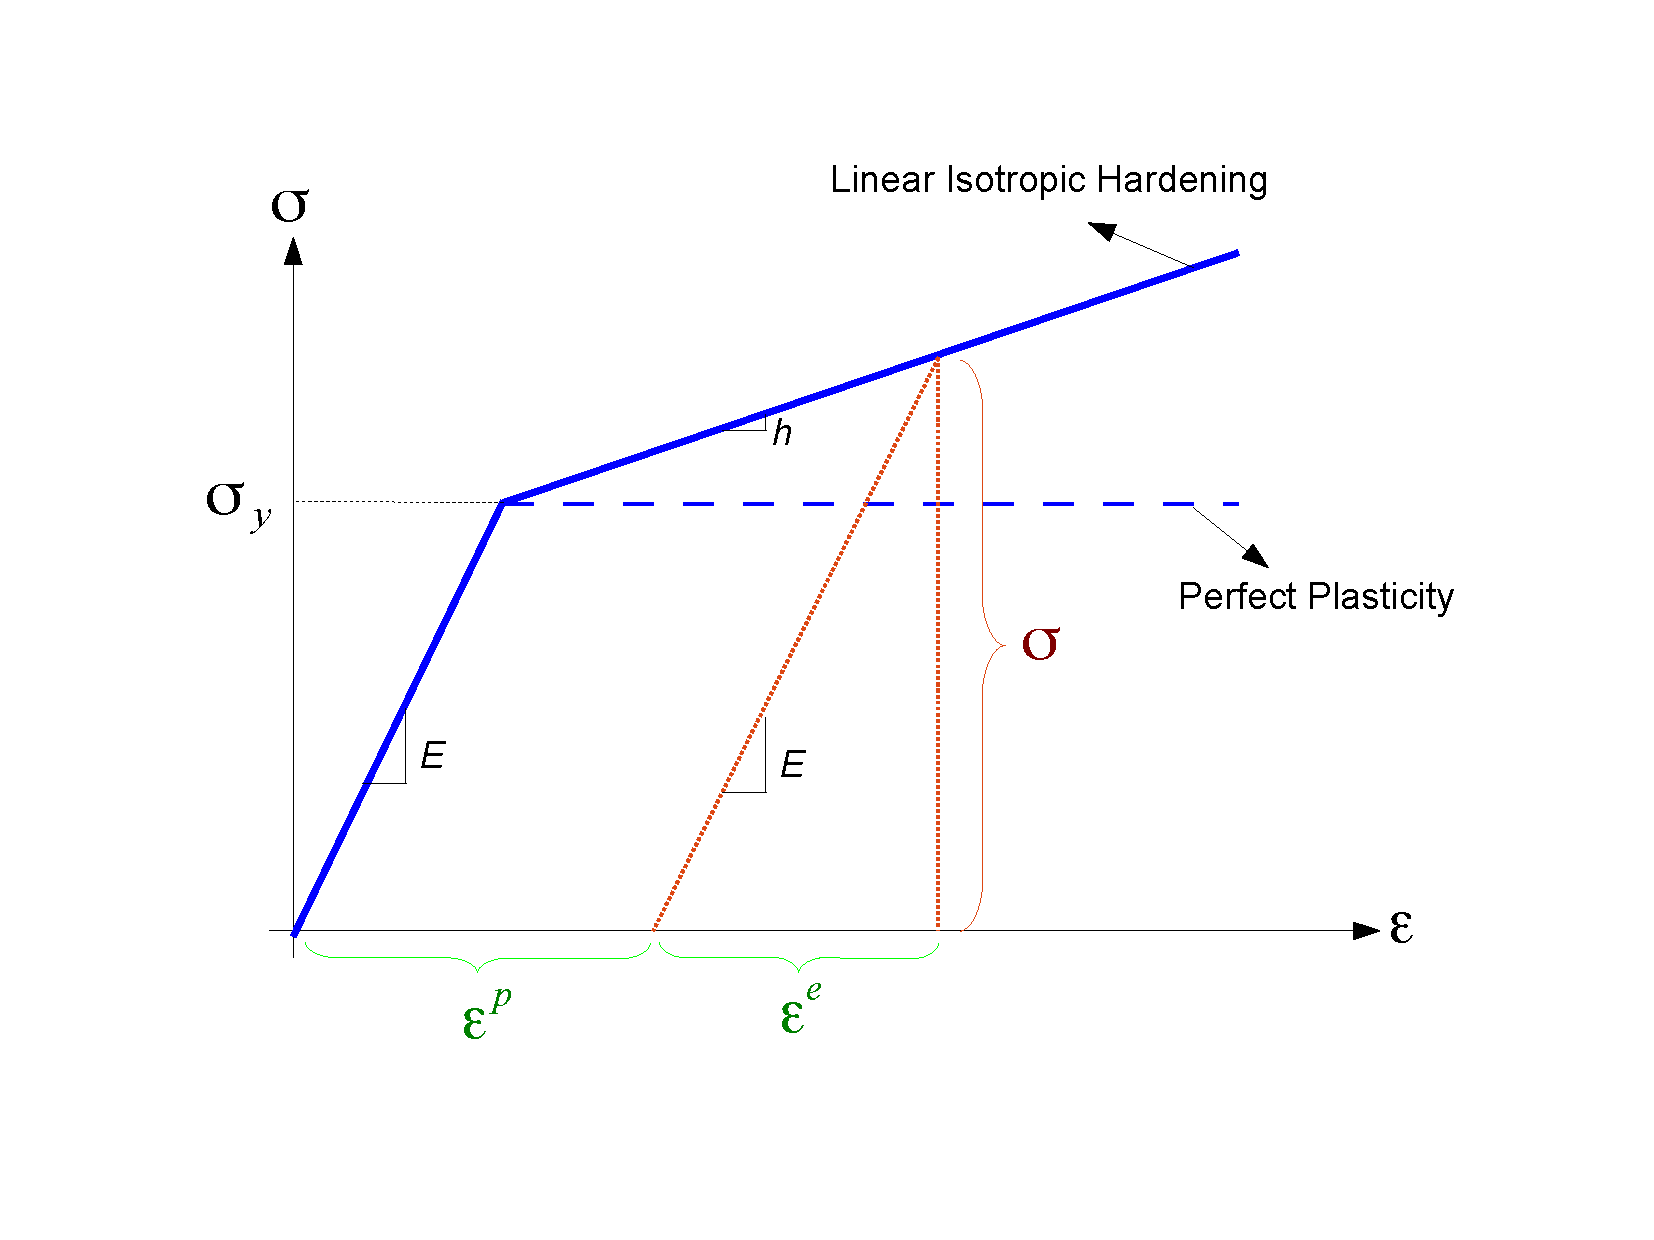
\includegraphics[scale=0.4, clip]{figures/isotropic_hardening_plasticity.pdf}}
   \caption{
    Stress-strain curve for the small-deformation plasticity with linear isotropic hardening.
   }
  \label{fig:smm:cl:Lin-strain-hard}
\end{figure}

\noindent In this class, the von Mises yield criterion is used. In the von Mises yield criterion, the yield is independent of the hydrostatic stress. Other yielding criteria such as Tresca and Gurson can be easily implemented in this class as well.

In the von Mises yield criterion, the hydrostatic stresses have no effect on the plasticity and consequently the yielding occurs when a critical elastic shear energy is achieved.

\begin{equation} \label{eqn:smm:constitutive:von Mises}
	f = \sigma_{\st{eff}} - \sigma_y = (\frac{3}{2} {\mat{\sigma}}^{\st{tr}} : {\mat{\sigma}}^{\st{tr}})^{1/2}-\sigma_y (\mat{\varepsilon}^p)
\end{equation}

\begin{equation} \label{eqn:smm:constitutive:yielding}
 	f < 0 \quad \textrm{Elastic deformation,} \qquad f = 0 \quad  \textrm{Plastic deformation}
\end{equation}

where $\sigma_y$ is the yield strength of the material which can be function of plastic strain in case of hardening type of materials and ${\mat{\sigma}}^{\st{tr}}$ is the deviatoric part of stress given by

\begin{equation} \label{eqn:smm:constitutive:deviatoric stress}
	{\mat{\sigma}}^{\st{tr}}=\mat{\sigma} - \frac{1}{3} trace(\mat{\sigma}) \mat {I}
\end{equation} 

After yielding $(f = 0)$, the normality hypothesis of plasticity determines the direction of plastic flow which is normal to the tangent to the yielding surface at the load point. Then, the tensorial form of the plastic constitutive equation using the von Mises yielding criterion (see equation 4.34) may be written as

\begin{equation} \label{eqn:smm:constitutive:plastic contitutive equation}
	\Delta {\mat{\varepsilon}}^p = \Delta p \frac {\partial{f}}{\partial{\mat \sigma}}=\frac{3}{2} \Delta p \frac{{\mat{\sigma}}^{\st{tr}}}{\sigma_{\st{eff}}}
\end{equation}

In these expressions, the direction of the plastic strain increment (or equivalently, plastic strain rate) is given by $\frac{{\mat{\sigma}}^{\st{tr}}}{\sigma_{\st{eff}}}$ while the magnitude is defined by the plastic multiplier $\Delta p$. This can be obtained using the \emph{consistency condition} which impose the requirement for the load point to remain on the yielding surface in the plastic regime.

\begin{table}[h]
\centering
  \begin{tabular}{| c | l | c |}
    \hline
    1 & Compute the trial stress & ${\mat{\sigma}}^{\st{tr}} = {\mat{\sigma}}_t + 2G\Delta \mat{\varepsilon} + \lambda trace(\Delta \mat{\varepsilon})\mat{I}$ \\[2ex] \hline
    2 & Check the Yielding criteria & $f = (\frac{3}{2} {\mat{\sigma}}^{\st{tr}} : {\mat{\sigma}}^{\st{tr}})^{1/2}-\sigma_y (\mat{\varepsilon}^p)$ \\[2ex] \hline
    3 & Compute the Plastic multiplier & \begin{tabular}{@{}c@{}c@{}} $d \Delta p = \frac{\sigma^{tr}_{eff} - 3G \Delta P^{(k)}- \sigma_y^{(k)}}{3G + h}		
$ \\ $\Delta p^{(k+1)}=\Delta p^{(k)}+ d\Delta p$ \\$\sigma_y^{(k+1)}=(\sigma_y)_t+ h\Delta p$ \end{tabular}\\ [2ex] \hline
    4 & Compute the plastic strain increment & $\Delta {\mat{\varepsilon}}^p = \frac{3}{2} \Delta p \frac{{\mat{\sigma}}^{\st{tr}}}{\sigma_{\st{eff}}}$ \\[2ex] \hline
    5 & Compute the stress increment & ${\Delta \mat{\sigma}} = 2G(\Delta \mat{\varepsilon}-\Delta \mat{\varepsilon}^p) + \lambda  trace(\Delta \mat{\varepsilon}-\Delta \mat{\varepsilon}^p)\mat{I}$ \\[2ex] \hline
    6 & Update the variables & \begin{tabular}{@{}c@{}} ${\mat{\varepsilon^p}}={\mat{\varepsilon}}^p_t+{\Delta {\mat{\varepsilon}}^p}$ \\    ${\mat{\sigma}}={\mat{\sigma}}_t+{\Delta \mat{\sigma}}$ \end{tabular}\\ [2ex] \hline     
    
  \end{tabular}
  \caption{Summary of the implementation procedure of small-deformation plasticity with linear isotropic hardening in \akantu}
  \label{table:equation for small-def plasticity with lin-iso-hardening}
\end{table}


Here, we summarize the implementation procedures for the
small-deformation plasticity with linear isotropic hardening. We use
an implicit integration technique called \emph{the radial return
  method} to obtain the plastic multiplier. This method has the
advantage of being unconditionally stable, however, the accuracy
remains dependent on the step size. The plastic parameters to indicate
in the material file are: \code{$\sigma_y$} (Yield stress) and
\code{h} (Hardening modulus). In addition, the elastic parameters need
to be defined as previously mentioned: \code{E} (Young's modulus),
\code{nu} (Poisson's ratio).


\subsection{Visco-Elasticity}

% Standard Solid rheological model, see [] J.C. Simo, T.J.R. Hughes,
% "Computational Inelasticity", Springer (1998), see Sections 10.2 and 10.3
Visco-elasticity is characterized by strain rate dependent
behavior. Moreover, when such a material undergoes a deformation it
dissipates energy. This dissipation results in a hysteresis loop in
the stress-strain curve at every loading cycle (see
Figure~\ref{fig:smm:cl:visco-elastic:hyst}). In principle, it can be
applied to many materials, since all materials exhibit a visco-elastic
behavior if subjected to particular conditions (such as high
temperatures).
\begin{figure}[!htb]
  \begin{center}

    \subfloat[]{
      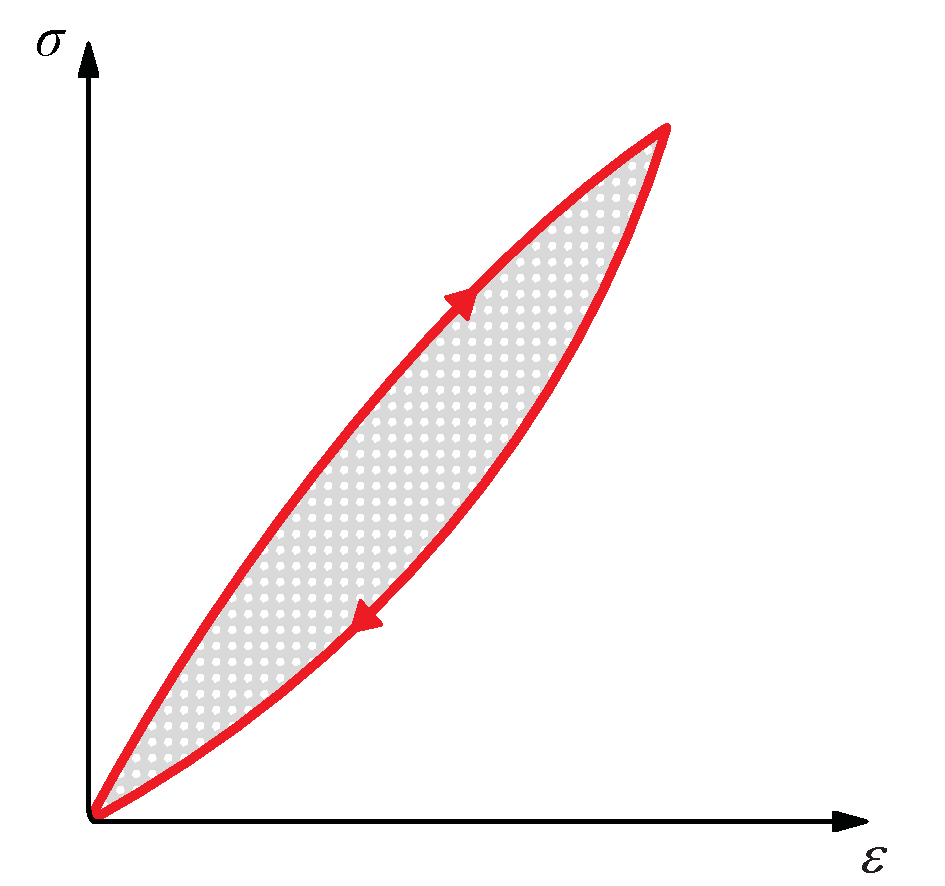
\includegraphics[width=0.4\textwidth,keepaspectratio=true]{figures/stress_strain_visco.pdf}
      \label{fig:smm:cl:visco-elastic:hyst}
    }
    \hspace{0.05\textwidth}
    \subfloat[]{
      \raisebox{0.025\textwidth}{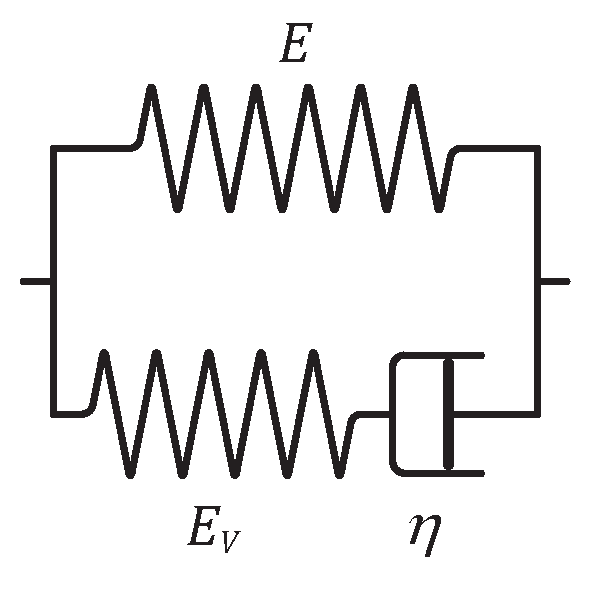
\includegraphics[width=0.3\textwidth,keepaspectratio=true]{figures/visco_elastic_law.pdf}}
      \label{fig:smm:cl:visco-elastic:model}
    }
    \caption{(a) Characteristic stress-strain behavior of a visco-elastic material with hysteresis loop and (b) schematic representation of the standard rheological linear solid visco-elastic model.}
    \label{fig:smm:cl:visco-elastic}
  \end{center}
\end{figure}
The standard rheological linear solid model (see Sections 10.2 and 10.3
of~\cite{simo92}) has been implemented in \akantu. This model results from the
combination of a spring mounted in parallel with a spring and a dashpot
connected in series, as illustrated in
Figure~\ref{fig:smm:cl:visco-elastic:model}. The advantage of this model is that
it allows to account for creep or stress relaxation. The equation that relates
the stress to the strain is (in 1D):
\begin{equation}
  \frac{d\epsilon(t)}{dt} = \left ( E + E_V \right ) ^ {-1} \cdot \left [ \frac{d\sigma(t)}{dt} + \frac{E_V}{\eta}\sigma(t) - \frac{EE_V}{\eta}\epsilon(t) \right ]
\end{equation}
where $\eta$ is the viscosity. The equilibrium condition is unique and
is attained in the limit, as $t \to \infty $. At this stage, the
response is elastic and depends on the Young's modulus $E$.  The
mandatory parameters for the material file are the following:
\code{rho} (density), \code{E} (Young's modulus), \code{nu} (Poisson's
ratio), \code{Plane\_Stress} (if set to zero plane strain, otherwise
plane stress), \code{eta} (dashpot viscosity) and \code{Ev} (stiffness
of the viscous element).

Note that the current standard linear solid model is applied only on the deviatoric part of the strain tensor. The spheric part of the strain tensor affects the stress tensor like an linear elastic material.

\subsection{Damage}

In the  simplified case of a  linear elastic and brittle  material, isotropic
damage can be represented by a scalar variable $d$, which varies from $0$ to $1$
for  no  damage  to  fully  broken  material  respectively.  The  stress-strain
relationship then becomes:
\begin{equation*}
  \mat{\sigma} = (1-d)\, \mat{C}:\mat{\varepsilon}
\end{equation*}

where  $\mat{\sigma}$,  $\mat{\varepsilon}$ are  the  Cauchy  stress and  strain
tensors, and $\mat{C}$ is the elastic stiffness tensor. This formulation relies
on the definition of an evolution law for the damage variable. In \akantu, many
possibilities exist and they are listed below.

\subsubsection{Marigo}
This damage evolution law is energy based as defined by Marigo \cite{marigo81a,
  lemaitre96a}. It is an isotropic damage law.
\begin{align}
  Y &= \frac{1}{2}\mat{\varepsilon}:\mat{C}:\mat{\varepsilon}\\
  F &= Y - Y_d - S d\\
  d &= \left\{
    \begin{array}{l l}
      \mathrm{min}\left(\frac{Y-Y_d}{S},\;1\right) & \mathrm{if}\; F > 0\\
      \mathrm{unchanged} & \mathrm{otherwise}
    \end{array}
  \right.
\end{align}
In this formulation, $Y$ is the strain energy release rate, $Y_d$ the
rupture criterion and $S$ the damage energy.  The non-local version of
this damage evolution law is constructed by averaging the energy $Y$.

\subsubsection{Mazars}
This law introduced by Mazars \cite{mazars84a} is a behavioral model to
represent damage evolution in concrete. The governing variable in this damage
law is the equivalent strain $\varepsilon_{\st{eq}} =
\sqrt{<\mat{\varepsilon}>_+:<\mat{\varepsilon}>_+}$, with $<.>_+$ the positive
part of the tensor.
The damage the is defined as:
\begin{align}
  D &= \alpha_t^\beta D_t + (1-\alpha_t)^\beta D_c\\
  D_t &= 1 - \frac{\kappa_0 (1- A_t)}{\varepsilon_{\st{eq}}} - A_t \exp^{-B_t(\varepsilon_{\st{eq}}-\kappa_0)}\\
  D_c &= 1 - \frac{\kappa_0 (1- A_c)}{\varepsilon_{\st{eq}}} - A_c
  \exp^{-B_c(\varepsilon_{\st{eq}}-\kappa_0)}\\
  \alpha_t &= \frac{\sum_{i=1}^3<\varepsilon_i>_+\varepsilon_{\st{nd}\;i}}{\varepsilon_{\st{eq}}^2}
\end{align}
With $\kappa_0$ the damage threshold, $A_t$ and $B_t$ the damage parameter in
traction, $A_c$ and $B_c$ the damage parameter in compression, $\beta$ is the
shear parameter. $\alpha_t$ is the coupling parameter between traction and
compression, the $\varepsilon_i$ are the eigenstrain and the
$\varepsilon_{\st{nd}\;i}$ are the eigenvalues of the strain if the material
were undamaged.

The coefficients $A$ and $B$ are the post-peak asymptotic
value and the decay shape parameters.


\subsection{Summary}\index{Material!List}

The list of all the materials available in Akantu is summarized in Tables \ref{tab:smm:cl:summary:list} as well as the keyword required for each material and the assosiated material properties.

\begin{table}[h!]
  \begin{center}
\begin{tabular}[c]{ m{3.5cm} | l | c | p{3.5cm} }
Material & Keyword & Parameter & Description \\
\hline
%%%%%%%%%%%%%%%%%
Linear elastic isotropic & \code{elastic} & -  & Table \ref{tab:smm:cl:summary:base}\\
\hline
%%%%%%%%%%%%%%%%%%
Linear elastic orthotropic  & \code{elastic\_orthotropic} & \code{Cij} & Tangent matrix coefficients (i,j = 1,2, ... voigt size ) \\
\hline
%%%%%%%%%%%%%%%%%%
Linear elastic anisotropic  & \code{elastic\_anisotropic} & \code{n1} & Direction of main material axis \\
 & & \code{n2} & Direction of secondary material axis \\
 & & \code{n3} & Direction of tertiery material axis \\
 & & \code{Cij} & Tangent matrix coefficients (i,j = 1,2, ... voigt size ) \\
 & & \code{alpha} & Proportion of viscous stress\\
\hline
%%%%%%%%%%%%%%%%%%
Neohookean (Finite-strain) \cite{Belytschko:2000} & \code{neohookean} & -  & Table \ref{tab:smm:cl:summary:base}\\
\hline
%%%%%%%%%%%%%%%%%%
Standard linear solid \cite{simo92} & \multirow{2}{*}{\code{sls\_deviatoric}} & - & Table \ref{tab:smm:cl:summary:base}\\
 & &  \code{Eta} & Viscosity\\
 & & \code{Ev} & Stiffness of the viscous element \\
\hline
%%%%%%%%%%%%%%%%%%
Elasto-plastic linear isotropic hardening & \code{plastic\_linear\_isotropic\_hardening}  & - & Table \ref{tab:smm:cl:summary:base}\\
 & &  \code{h} & Hardening modulus\\
 & &  \code{sigma\_y} & Yielding stress\\
\hline
%%%%%%%%%%%%%%%%%%
Visco-plastic & \code{visco\_plastic}  & - & Table \ref{tab:smm:cl:summary:base}\\
 & &  \code{rate} & Rate sensitivity component\\
 & &  \code{edot0} & Reference strain rate\\
 & &  \code{ts} & Time \\
\hline
\end{tabular}
\end{center}
  \caption{List of material properties with their corresponding keywords and material parameters.}
  \label{tab:smm:cl:summary:list}
\end{table}

\vspace{0.5cm}

In addition to the properties presented in Table \ref{tab:smm:cl:summary:list}, every material also has the parameter ''\code{rho}`` which corresponds to the density. The properties listed in Table  \ref{tab:smm:cl:summary:base} correspond to the parameters required to describe a linear elastic isotropic material, however those parameters are also commun to most of the materials available as previously described in Table \ref{tab:smm:cl:summary:list}.

\begin{table}[h!]
  \begin{center}
\begin{tabular}[c]{  l | p{6.5cm} }\label{tab:smm:cl:summary:base}
Parameter & Description \\
\hline
%%%%%%%%%%%%%%%%%
\code{rho}  & Density\\
\code{E}  & Young's modulus\\
\code{nu}  & Poisson's ratio\\
\code{Plane\_Stress} & Plane stress simplification (only 2D problems)\\
\hline
\end{tabular}
\end{center}
  \caption{List of material parameters shared my most materials}
  \label{tab:smm:cl:summary:base}
\end{table}

%%% Local Variables:
%%% mode: latex
%%% TeX-master: "manual"
%%% End:
}{}

\IfFileExists{manual-cohesive_laws.tex}{\subsection{Cohesive laws}
\label{sec:cohesive-laws}

\subsubsection{Linear Irreversible Law\matlabel{ssect:smm:cl:coh-snozzi}}

\begin{figure}[!hbt]
  \centering
  \subfloat[Linear]{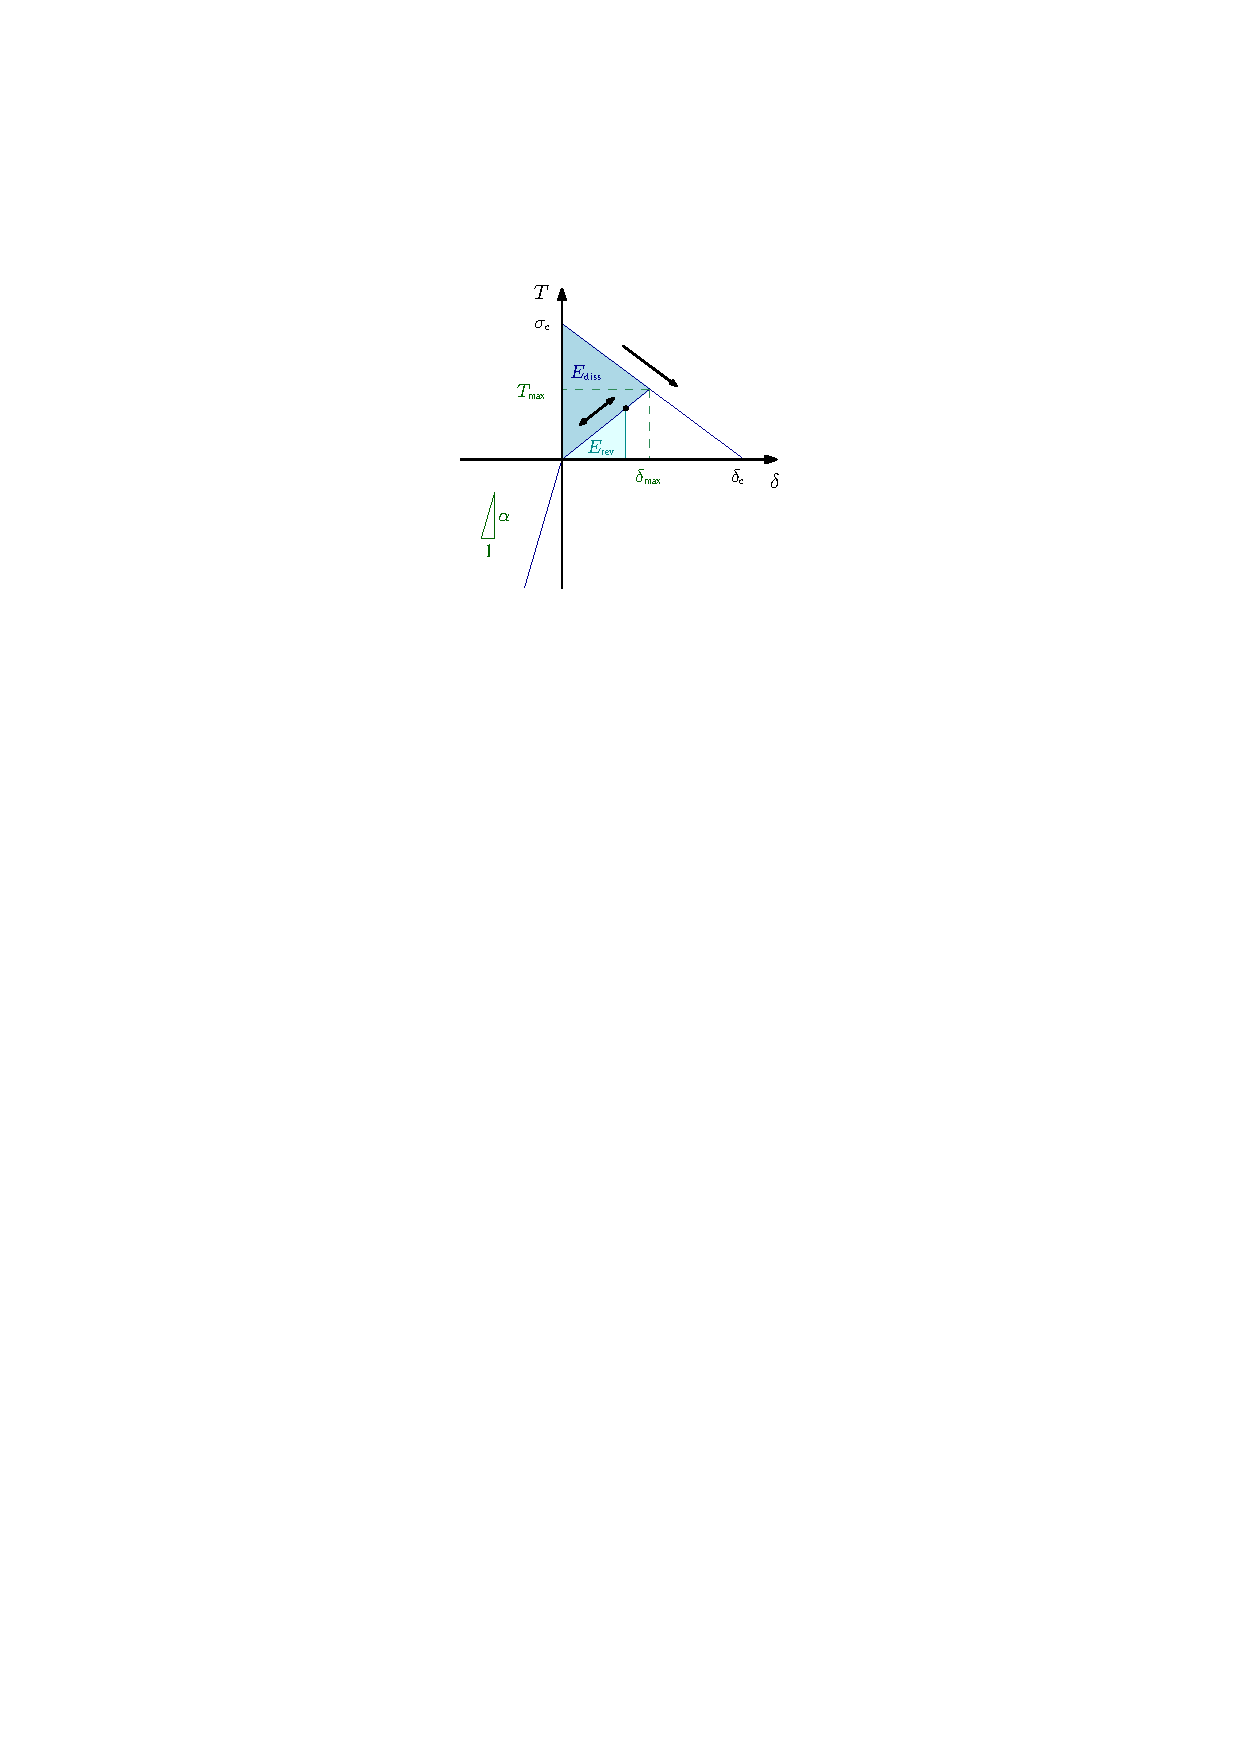
\includegraphics[width=0.4\textwidth]{figures/linear_cohesive_law}}
  \qquad
  \subfloat[Bilinear]{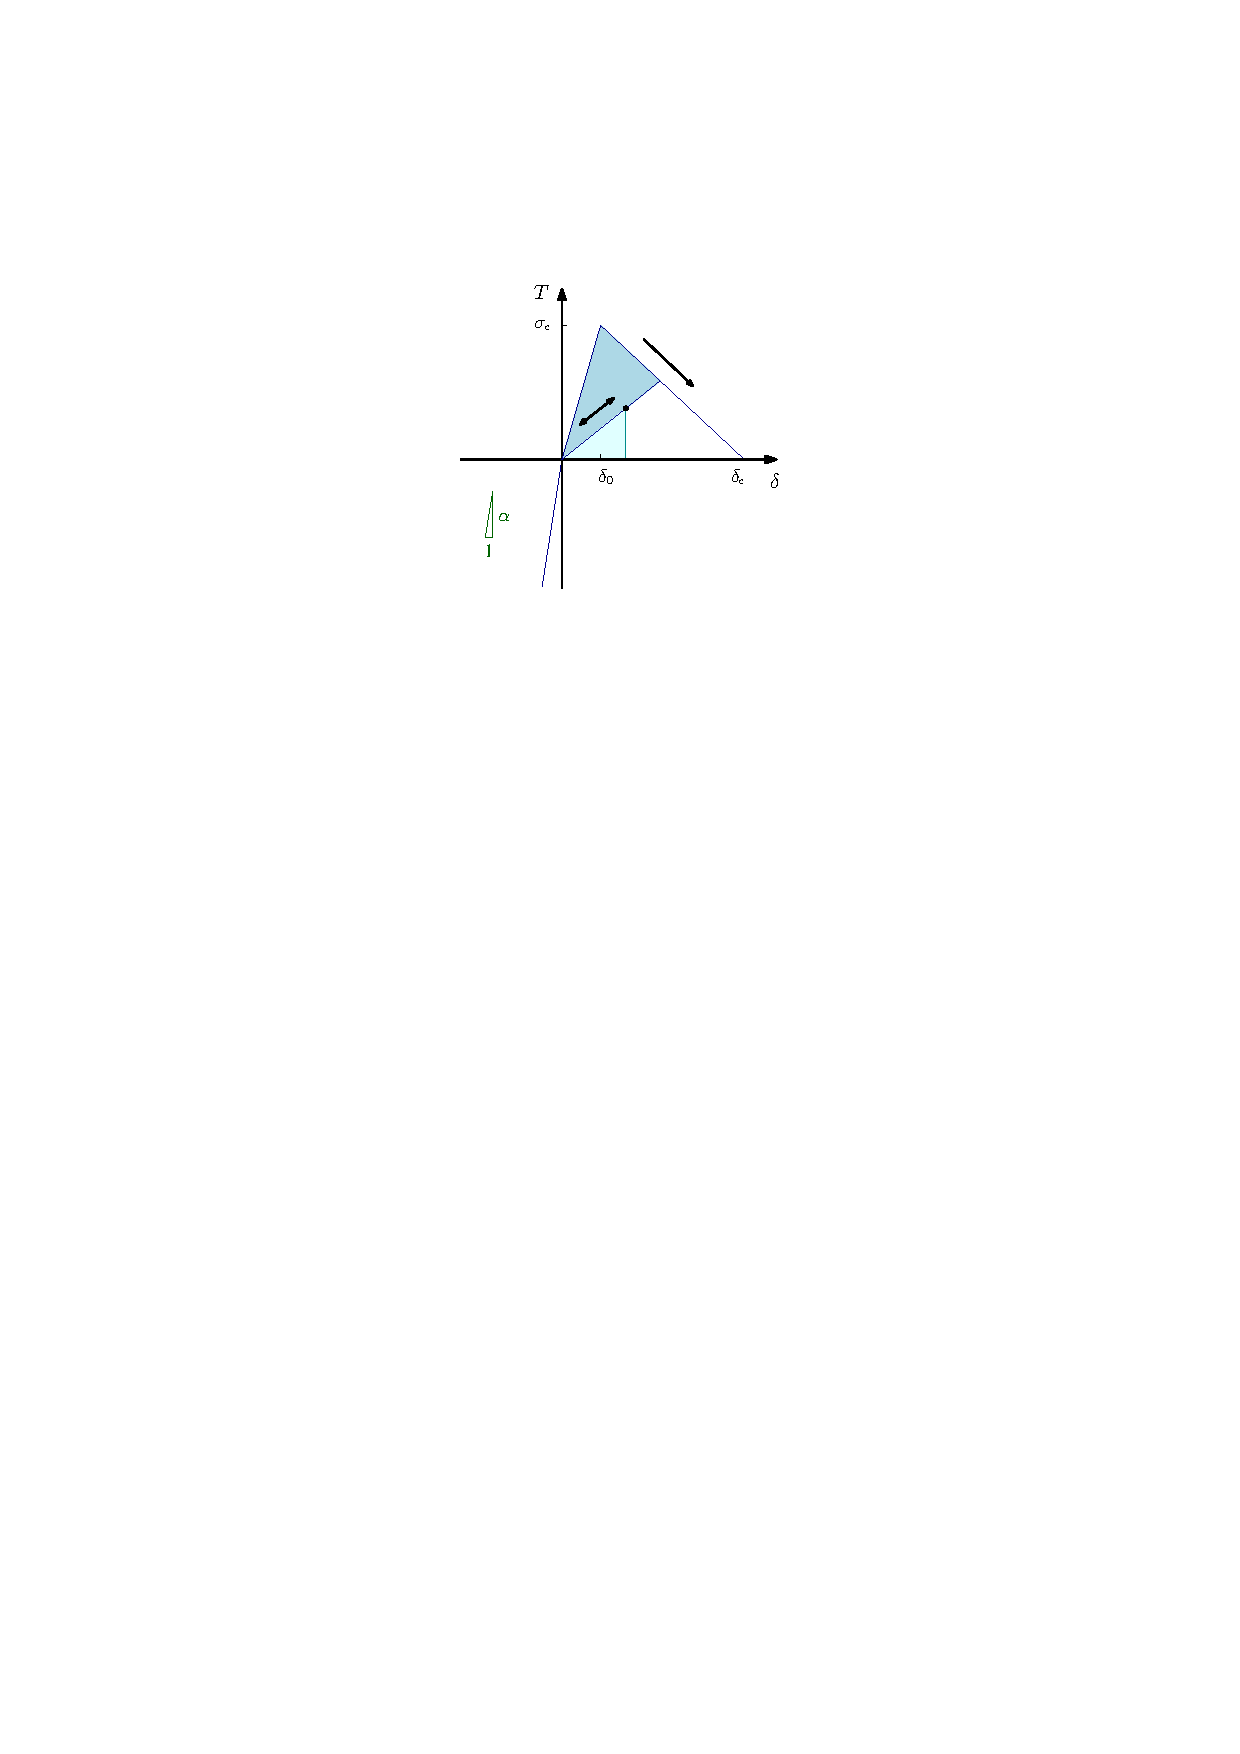
\includegraphics[width=0.4\textwidth]{figures/bilinear_cohesive_law}}
  \caption{Irreversible cohesive laws for explicit simulations.}
  \label{fig:smm:coh:linear_cohesive_law}
\end{figure}

\akantu includes the Snozzi-Molinari~\cite{snozzi_cohesive_2013}
linear irreversible cohesive law (see
Figure~\ref{fig:smm:coh:linear_cohesive_law}). It is an extension to
the Camacho-Ortiz~\cite{camacho_computational_1996} cohesive law in
order to make dissipated fracture energy path-dependent. The concept
of free potential energy is dropped and a new independent parameter
$\kappa$ is introduced:
\begin{equation}
  \kappa = \frac{G_\mathrm{c, II}}{G_\mathrm{c, I}}
\end{equation}

where $G_\mathrm{c, I}$ and $G_\mathrm{c, II}$ are the
necessary works of separation per unit area to open completely a
cohesive zone under mode I and mode II, respectively. Their model yields to the
following equation for cohesive tractions $\vec{T}$ in case of crack
opening ${\delta}$:
\begin{equation}
  \label{eq:smm:coh:tractions}
  \vec{T} = \left( \frac{\beta^2}{\kappa} \Delta_\mathrm{t} \vec{t} +
    \Delta_\mathrm{n} \vec{n} \right)
  \frac{\sigma_\mathrm{c}}{\delta}
  \left( 1- \frac{\delta}{\delta_\mathrm{c}} \right)
  = \hat{\vec T}\,
  \frac{\sigma_\mathrm{c}}{\delta}
  \left( 1- \frac{\delta}{\delta_\mathrm{c}} \right)
\end{equation}

where $\sigma_\mathrm{c}$ is the material strength along the fracture,
$\delta_\mathrm{c}$ the critical effective displacement after which
cohesive tractions are zero (complete decohesion), $\Delta_\mathrm{t}$
and $\Delta_\mathrm{n}$ are the tangential and normal components of
the opening displacement vector $\vec{\Delta}$, respectively. The
parameter $\beta$ is a weight that indicates how big the tangential
opening contribution is. The effective opening displacement is:
\begin{equation}
  \delta = \sqrt{\frac{\beta^2}{\kappa^2} \Delta_\mathrm{t}^2 +
    \Delta_\mathrm{n}^2}
\end{equation}
In case of unloading or reloading $\delta < \delta_\mathrm{max}$,
tractions are calculated as:
\begin{align}
  T_\mathrm{n} &= \Delta_\mathrm{n}\,
  \frac{\sigma_\mathrm{c}}{\delta_\mathrm{max}}
  \left( 1- \frac{\delta_\mathrm{max}}{\delta_\mathrm{c}} \right) \\
  T_\mathrm{t} &= \frac{\beta^2}{\kappa}\, \Delta_\mathrm{t}\,
  \frac{\sigma_\mathrm{c}}{\delta_\mathrm{max}}
  \left( 1- \frac{\delta_\mathrm{max}}{\delta_\mathrm{c}} \right)
\end{align}
so that they vary linearly between the origin and the maximum attained
tractions. As shown in Figure~\ref{fig:smm:coh:linear_cohesive_law},
in this law, the dissipated and reversible energies are:
\begin{align}
  E_\mathrm{diss} &= \frac{1}{2} \sigma_\mathrm{c}\, \delta_\mathrm{max}\\[1ex]
  E_\mathrm{rev} &= \frac{1}{2} T\, \delta
\end{align}
Moreover, a damage parameter $D$ can be defined as:
\begin{equation}
  D = \min \left(
    \frac{\delta_\mathrm{max}}{\delta_\mathrm{c}},1 \right)
\end{equation}
which varies from 0 (undamaged condition) and 1 (fully
damaged condition). This variable can only increase because damage is
an irreversible process. A simple penalty contact model has been incorporated
in the cohesive law so that normal tractions can be returned in
case of compression:
\begin{equation}
  T_\mathrm{n} = \alpha \Delta_\mathrm{n} \quad\text{if
    $\Delta_\mathrm{n} < 0$}
\end{equation}
where $\alpha$ is a stiffness parameter that defaults to zero. The
relative contact energy is equivalent to reversible energy but in
compression.

The material name of the linear decreasing cohesive law  is
\code{material\_cohesive\_linear} and its parameters with their
respective default values are:
\begin{itemize}
\item \code{sigma\_c}: 0
\item \code{delta\_c}: 0
\item \code{beta}: 0
\item \code{G\_c}: 0
\item \code{kappa}: 1
\item \code{penalty}: 0
\end{itemize}
where \code{G\_c} corresponds to $G_\mathrm{c, I}$. A random number
generator can be used to assign a random $\sigma_\mathrm{c}$ to each
facet following a given distribution (see
Section~\ref{sect:smm:CL}). Only one parameter between \code{delta\_c}
and \code{G\_c} has to be specified. For random $\sigma_\mathrm{c}$
distributions, the chosen parameter of these two is kept fixed and the
other one is varied.

The bilinear constitutive law works exactly the same way as the linear
one, except for the additional parameter \code{delta\_0} that by
default is zero. Two examples for the extrinsic and intrinsic cohesive
elements and also an example to assign different properties to
intergranular and transgranular cohesive elements can be found in
the folder \code{\examplesdir/cohesive\_element/}.

\subsubsection{Linear Cohesive Law with Fatigue\matlabel{ssect:smm:cl:coh-fatigue}}

This law represents a variation of the linear irreversible cohesive
law of the previous section, that removes the hypothesis of elastic
unloading-reloading cycles. With this law, some energy is dissipated
also during unloading and reloading with hysteresis. The
implementation follows the work of~\cite{nguyen2001}. During the
unloading-reloading cycle, the traction increment is computed as
\begin{equation}
  \dot{T} =
  \begin{cases}
    K^- \, \dot{\delta} & \text{if $\dot{\delta} < 0$} \\
    K^+ \, \dot{\delta} & \text{if $\dot{\delta} > 0$} \\
  \end{cases}
\end{equation}
where $\dot{\delta}$ and $\dot{T}$ are respectively the effective
opening displacement and the cohesive traction increments with respect
to time, while $K^-$ and $K^+$ are respectively the unloading and
reloading incremental stiffness. The unloading path is linear and
results in an unloading stiffness
\begin{equation}
  K^- = \frac{T_\mathrm{max}}{\delta_\mathrm{max}}
\end{equation}
where $T_\mathrm{max}$ and $\delta_\mathrm{max}$ are the maximum
cohesive traction and the effective opening displacement reached
during the precedent loading phase. The unloading stiffness remains
constant during the unloading phase. On the other hand the reloading
stiffness increment $\dot{K}^+$ is calculated as
\begin{equation}
  \dot{K}^+ =
  \begin{cases}
    - K^+ \, \dot{\delta} / \delta_\mathrm{f} & \text{if $\dot{\delta}
      > 0$} \\
    \left( K^+ - K^- \right) \, \dot{\delta} / \delta_\mathrm{f} &
    \text{if $\dot{\delta} < 0$}
  \end{cases}
\end{equation}
where $\delta_\mathrm{f}$ is a material parameter. During unloading
the stiffness $K^+$ tends to $K^-$, while during reloading $K^+$ gets
decreased at every time step. If the cohesive traction during
reloading exceeds the upper limit given by
equation~\eqref{eq:smm:coh:tractions}, it is recomputed following the
behavior of the linear decreasing cohesive law for crack opening.

\subsubsection{Exponential Cohesive Law\matlabel{ssect:smm:cl:coh-exponential}}

Ortiz and Pandolfi proposed this cohesive law in 1999~\cite{ortiz1999}.  The
traction-opening equation for this law is as follows:
\begin{equation}
  \label{eq:exponential_law}
  T = e \sigma_c \frac{\delta}{\delta_c}e^{-\delta/ \delta_c}
\end{equation}
This equation is plotted in Figure~\ref{fig:smm:CL:ECL}. The term
$\partial{\vec{T}}/ \partial{\delta}$ of
equation~\eqref{eq:cohesive_stiffness} after the necessary derivation
can expressed as
\begin{equation}
  \label{eq:tangent_cohesive}
  \frac{\partial{\vec{T}}} {\partial{\delta}} = \hat{\vec{T}} \otimes
  \frac                       {\partial{(T/\delta)}}{\partial{\delta}}
  \frac{\hat{\vec{T}}}{\delta}+ \frac{T}{\delta}  \left[ \beta^2 \mat{I} +
  \left(1-\beta^2\right) \left(\vec{n} \otimes \vec{n}\right)\right]
\end{equation}
where
\begin{equation}
  \frac{\partial{(T/ \delta)}}{\partial{\delta}} = \left\{\begin{array} {l l}
      -e  \frac{\sigma_c}{\delta_c^2  }e^{-\delta  /  \delta_c} &  \quad  if
      \delta \geq \delta_{max}\\
      0 & \quad if \delta < \delta_{max}, \delta_n > 0
    \end{array} \right.
\end{equation}


\begin{figure}[!htb]
  \begin{center}
    \includegraphics[width=0.6\textwidth,keepaspectratio=true]{figures/cohesive_exponential.pdf}
    \caption{Exponential cohesive law}
    \label{fig:smm:CL:ECL}
  \end{center}
\end{figure}


%%% Local Variables:
%%% mode: latex
%%% TeX-master: "manual"
%%% End:
}{}


%%% Local Variables:
%%% mode: latex
%%% TeX-master: "manual"
%%% End:
